% Analyse
\section{Analyse}

% User Szenarien
\subsection{User Szenarien}
\label{kort-user-szenarien}

Um die Anforderungen an die App genauer abschätzen zu können, wurden im Vorfeld der Implementierung einige Szenarien erstellt.

\subsubsection{Szenario 1: Zeitvertreib an der Bushaltestelle}

Simon muss 15 Minuten an der Bushaltestelle auf den nächsten Bus warten.
Um sich die Wartezeit zu verkürzen, nimmt er sein Smartphone hervor und startet die \kort{}-Applikation.

Die App hat ihn bereits lokalisiert und zeigt ihm offene \brand{OpenStreetMap}-Aufträge in der Nähe, wahlweise als Liste oder auf der Karte an.
Für die Aufträge werden Simon verschiedene Belohnungen angeboten, abhängig vom Schwierigkeitsgrad der Aufgabe.

Simon entscheidet sich für einen Auftrag mit mittlerer Belohnung.
Die App zeigt ihm den Weg zum Auftrag und erklärt, was zu tun ist.
Beim Auftrag handelt es sich um einen fehlenden Strassennamen.

Als Simon vor Ort ist, findet er sehr schnell ein Strassenschild.
Er gibt den Namen in der App ein wofür er bereits 10 Punkte erhält.
Da er zusätzlich sogar noch ein Foto hochlädt, bekommt er weitere 5 Punkte.

Der Auftrag ist somit für ihn erledigt, was ihm entsprechend von der App mitgeteilt wird.
Danach verschwindet der Auftrag aus seiner Auftragsliste und von der Karte.

\textbf{Ziele}
\begin{itemize}
\item Zeitvertreib
\item Punkte sammeln
\item Daten verbessern
\end{itemize}

\subsubsection{Szenario 2: Validieren}

Andy sitzt im Zug und langweilt sich.
Er öffnet die \kort{}-App im Indoor-Modus und sieht sich die Liste der zu validierenden Lösungsvorschläge an. 
Er sortiert die Liste, um diejenigen Einträge zu sehen, welche nur noch einen Review benötigen, um an \brand{OpenStreetMap} gesendet werden zu können.

Er öffnet einen Vorschlag für einen fehlenden Strassennamen in der Umgebung.
Er kennt zwar die Gegend ist sich aber nicht 100\% sicher ob der Name stimmt.
Um sicherzugehen, öffnet er das angehängte Bild.
Das Bild zeigt ein Strassenschild, welches mit dem eingegeben Namen übereinstimmt
Andy bestätigt dann die Änderung und schliesst den Bug damit ab.

\cleardoublepage
\textbf{Ziele}
\begin{itemize}
\item Schnell und einfach geeignete Einträge zum Validieren finden
\item Qualität der Änderungen sicherstellen
\end{itemize}

\subsubsection{Szenario 3: Erster Kontakt zur App}

Über den Kurznachrichtendienst Twitter sieht Monika, dass ihre Kollegin gerade das erste mal \kort{} gestartet hat.
Als sie auf den Link klickt öffnet sich ihr Browser und die App wird angezeigt.
Da es sich um ihren ersten Besuch auf der Seite handelt, wird ihr kurz erklärt um was es geht.

Danach sieht sie die Karte mit den vorhandenen Fehlereinträgen.
Bevor sie einen Eintrag bearbeiten kann, muss sie sich anmelden.
Sie wählt dazu einen Benutzernamen und wird anschliessend auf die Seite von Google weitergeleitet, um sich anzumelden.
Nach dem erfolgreichen Login wird Monika zurück zur \kort{}-App geleitet, wo sie beginnen kann, die ersten Aufträge zu erfüllen.

\textbf{Ziele}
\begin{itemize}
\item Direkt ersichtlich, was die App kann
\item Schneller Einstieg
\item Einfache Anmeldung (keine Registrierung!)
\item Benutzerführung durch die Funktionen
\end{itemize}

\subsubsection{Szenario 4: Highscore-Anwärter}

Edi benutzt schon seit einiger Zeit die \kort{}-App und hat in seinem Revier bereits den zweiten Platz der Highscore erreicht.
Seine Platzierung überprüft er regelmässig in der App.

Heute möchte er endlich die Spitze erklimmen und den "`Leader"'-Badge erhalten.
Dazu hat er sich einige Aufträge ausgesucht, welche er der Reihe nach bearbeiten will.
Bei jedem Auftrag sieht Edi, wie viele Punkte er sammeln kann.

Nachdem er den 5. Auftrag erfolgreich erledigt hat, erhält er eine Benachrichtigung, dass er den "`Leader"'-Badge erhalten hat.
Auch in der Rangliste steht Edi nun zuoberst.

\textbf{Ziele}
\begin{itemize}
\item Einfach mehrere Aufträge nacheinander ausführen
\item Badges sammeln
\item Highscore anzeigen
\item Erster Rang erreichen
\end{itemize}

% Paper-Prototype
\subsection{Paper-Prototype}
% Subfigure counter zuruecksetzen
\setcounter{subfigure}{0}

Aus den gesetzten Projektzielen und den Anforderungen der erstellten Szenarien (siehe Abschnitt \ref{kort-user-szenarien}) wurde vor der Implementation der Oberfläche ein Paper-Prototype des GUI-Designs erstellt.
Der Prototype besteht aus vier Hauptmasken und einem Overlay für den Login.

\subsubsection{Overlay: Login}
Beim ersten Starten der \gls{WebApp} erhält man die Möglichkeit sich über verschiedene Dienste anzumelden.
Mit einem Klick auf den jeweiligen Anbieter, wird man zu diesem weitergeleitet und kann sich dort anmelden.

\begin{figure}[H]
\subfigure[Login - Anbieterauswahl]{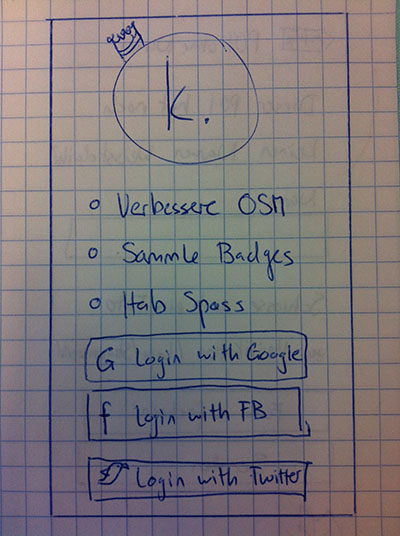
\includegraphics[width=0.43\textwidth]{images/paperprototype/kort-pp-startscreen}}
\hfill
\subfigure[Login - Loginformular des jeweiligen Anbieters]{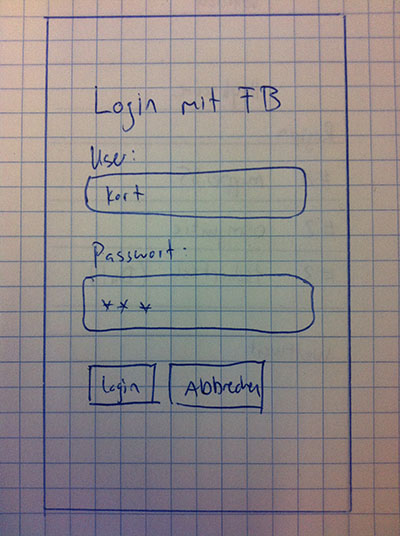
\includegraphics[width=0.43\textwidth]{images/paperprototype/kort-pp-login}}
\end{figure}

\cleardoublepage
\subsubsection{Maske: Aufträge}
Nachdem sich der Benutzer erfolgreich angemeldet hat, erscheint die Maske mit den Aufträgen.
Darauf werden die vorhandenen Fehler auf einer Karte angezeigt.
Es werden jeweils nur die Fehler angezeigt, welche sich in unmittelbarer Nähe des eigenen Standorts befinden.
Die Fehler werden mit einer Markierung auf der Karte dargestellt.

Durch Anklicken einer solchen Markierung öffnet sich die Detailansicht des Fehlers, wo sich der Fehler direkt beheben lässt.
Neben der Möglichkeit, einen Lösungstext einzugeben, soll es auch möglich sein, ein Beweis-Foto hochzuladen.
Mit einem Klick auf den Senden-Knopf schliesst sich die Detailansicht und man gelangt zur Karte mit den Aufträgen zurück.

\begin{figure}[H]
\subfigure[Aufträge - Karte mit Fehlern]{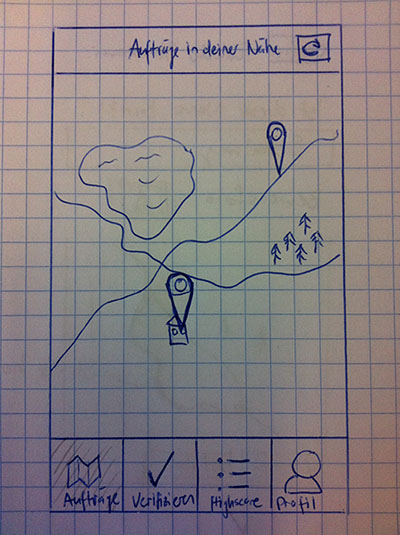
\includegraphics[width=0.43\textwidth]{images/paperprototype/kort-pp-bugs}}
\hfill
\subfigure[Aufträge - Detailansicht eines Fehlers]{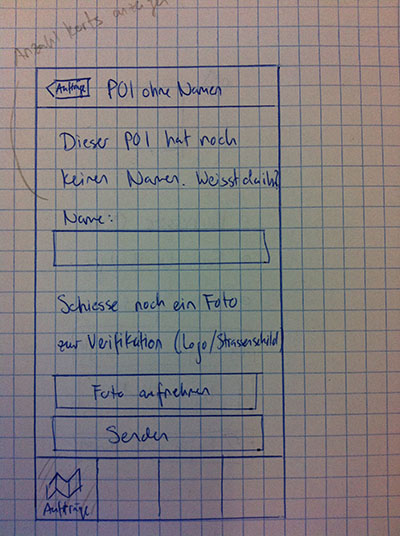
\includegraphics[width=0.43\textwidth]{images/paperprototype/kort-pp-fix}}
\end{figure}

\cleardoublepage
\subsubsection{Maske: Verifizieren}
Auf der Verifikationsmaske werden die bereits gelösten Fehler in der Nähe angezeigt.
Sie sind gruppiert nach Anzahl nötigen Verifikationen, um sie an \brand{OpenStreetMap} zurückzusenden.

Per Klick auf einen Eintrag öffnet sich die Verifikationsmaske.
Darin wird der Fehlerlösungstext und das Beweis-Foto angezeigt.
Zusätzlich wird das betroffene \brand{OpenStreetMap}-Objekt auf einer Karte angezeigt.
Man hat die Möglichkeit, die Problemlösung als \emph{Korrekt} oder \emph{Falsch} zu bewerten.

\begin{figure}[H]
\subfigure[Verifizieren - Liste mit Fehlerlösungen]{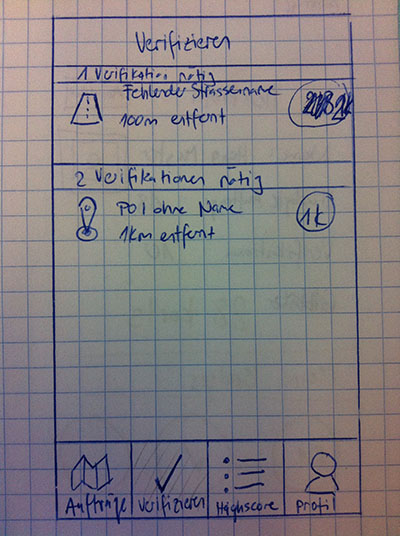
\includegraphics[width=0.43\textwidth]{images/paperprototype/kort-pp-verify}}
\hfill
\subfigure[Verifizieren - Detailansicht einer Fehlerlösung]{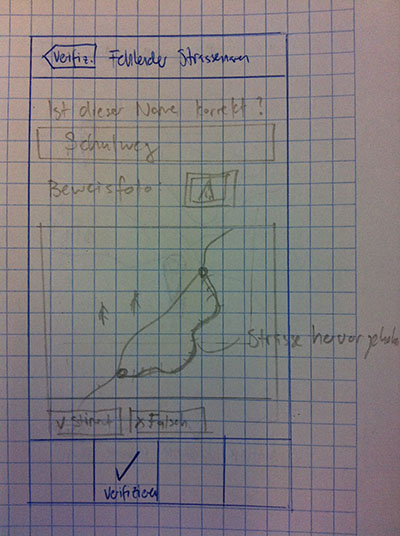
\includegraphics[width=0.43\textwidth]{images/paperprototype/kort-pp-verify_detail}}
\end{figure}

\cleardoublepage
\subsubsection{Maske: Highscore}
In der Highscore-Maske kann man sich mit anderen Spielern messen.
Man sieht seine eigene Platzierung und die der anderen Spieler.
Es werden Highscores für verschiedene Kategorien (z.B. regional, weltweit) angezeigt.

\subsubsection{Maske: Profil}
Im Profil werden die Eckdaten des eigenen Benutzers angezeigt.
Dazu gehören die Anzahl der gelösten Aufträge und die Anzahl der getätigten Verifikationen.
Zusätzlich werden die Gesamtanzahl der gesammelten Punkte und die gewonnenen Badges ausgewiesen.
Auf der Profil-Maske kann sich der Benutzer von der App abzumelden.

\begin{figure}[H]
\subfigure[Highscore]{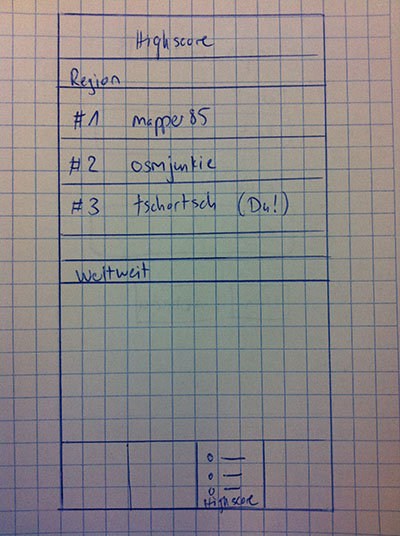
\includegraphics[width=0.43\textwidth]{images/paperprototype/kort-pp-highscore}}
\hfill
\subfigure[Profil]{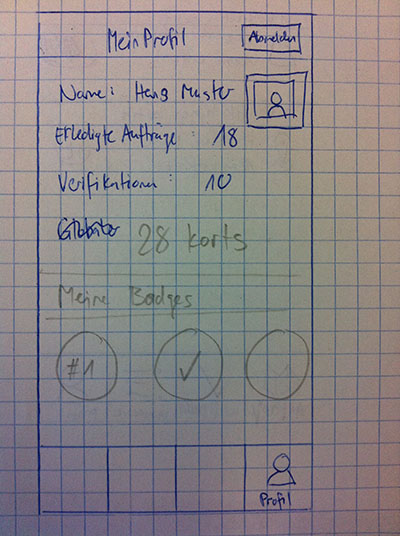
\includegraphics[width=0.43\textwidth]{images/paperprototype/kort-pp-profile}}
\end{figure}